%% Adaptado de 
%% http://www.ctan.org/tex-archive/macros/latex/contrib/IEEEtran/
%% Traduzido para o congresso de IC da USP
%%*****************************************************************************
% Não modificar

\documentclass[twoside,conference,a4paper]{IEEEtran}

%******************************************************************************
% Não modificar
\usepackage{IEEEtsup} % Definições complementares e modificações.
\usepackage[latin1,utf8]{inputenc} % Disponibiliza acentos.
\usepackage[english,brazil]{babel}
%\usepackage[brazil,brazilian]{babel}
%% Disponibiliza Inglês e Português do Brasil.
\usepackage{latexsym,amsfonts,amssymb} % Disponibiliza fontes adicionais.
\usepackage{theorem} 
\usepackage[cmex10]{amsmath} % Pacote matemático básico 
\usepackage{url} 
%\usepackage[portuges,brazil,english]{babel}
\usepackage{graphicx}
\usepackage{amsmath}
\usepackage{amssymb}
\usepackage{color}
\usepackage[pagebackref=true,breaklinks=true,letterpaper=true,colorlinks,bookmarks=false]{hyperref}
\usepackage[tight,footnotesize]{subfigure} 
\usepackage[noadjust]{cite} % Disponibiliza melhorias em citações.
\usepackage{algorithmic}
\usepackage{algpseudocode} 
\usepackage{algorithm}


%%*****************************************************************************

\begin{document}
\selectlanguage{brazil}
\renewcommand{\IEEEkeywordsname}{Palavras-chave}

%%*****************************************************************************

\urlstyle{tt}
% Indicar o nome do autor e o curso/nível (grad-mestrado-doutorado-especial)
\title{Project 3 - XX - AI}
\author{%
 \IEEEauthorblockN{Christian Maekawa\,\IEEEauthorrefmark{1}}
 \IEEEauthorblockA{\IEEEauthorrefmark{1}%
                   RA: XXX \\
                   E-mail: XXX@ic.unicamp.br}
 \IEEEauthorblockN{Giovane de Morais\,\IEEEauthorrefmark{1}}
 \IEEEauthorblockA{\IEEEauthorrefmark{1}%
                   RA: XXX \\
                   E-mail: g192683@dac.unicamp.br}
 \IEEEauthorblockN{Maísa Silva\,\IEEEauthorrefmark{1}}
 \IEEEauthorblockA{\IEEEauthorrefmark{1}%
                   RA: XXX \\
                   E-mail: XXX@ic.unicamp.br}
 \IEEEauthorblockN{Matteus Vargas\,\IEEEauthorrefmark{1}}
 \IEEEauthorblockA{\IEEEauthorrefmark{1}%
                   RA: XXX \\
                   E-mail: XXX@ic.unicamp.br}
 \IEEEauthorblockN{Stéfani Fernandes\,\IEEEauthorrefmark{1}}
 \IEEEauthorblockA{\IEEEauthorrefmark{1}%
                   RA: XXX \\
                   E-mail: XXX@ic.unicamp.br}
}

%%*****************************************************************************

\maketitle

%%*****************************************************************************
% Resumo do trabalho
\begin{abstract}

\end{abstract}

% Indique três palavras-chave que descrevem o trabalho
\begin{IEEEkeywords}
 Palavras-chave
\end{IEEEkeywords}

%%*****************************************************************************
% Modifique as seções de acordo com o seu projeto

\section{Introdução}

O presente relatório apresenta a descrição das estratégias adotadas para a resolução do Projeto 3 da disciplina Introdução à Inteligência Artificial, ministrada no primeiro semestre de 2020 pela professora Dra. Esther Luna Colombini.


A seção II 

A seção III 

A seção IV 

A seção V, por fim, apresenta as conclusões da obra.

\section{Especificação do Problema}


\section{XX}

XXXX

\section{Metodologia}
A projeto \textit{CAPTCHA}, foi construído com base em uma arquitetura de redes neurais em \textit{Deep Learning} com cinco camadas convolucionais, sendo uma entrada e uma saída acrescido de três \textit{hidden layers}, mais especificamente Conv2D com os parâmetros de \textit{padding = ``same''} e ativação ``relu'' (os detalhes técnicos de implementação como a explicação dos parâmetros serão melhor descritos em Detalhes da Implementação). Abaixo, será descrito os procedimentos que compõem o projeto que são o processamento, reconhecimento e quebra das imagens alfanuméricas CAPTCHA. O processo inclui pré-processamento de dados de entrada, estruturação da rede e predição.

\subsection{Pré-Processamento}

Operações de pré-processamento, como alterações nas dimensões da imagem, ajuste nos canais de cores, identificação e mitigação de ruídos. Tais operações podem normalizar os dados para determinados padrões, o que costuma gerar melhoras significativas na rede neural.

O tamanho de todas as imagens do \textit{dataset}, sem excessão, é de 50 x 200 pixels (veja o exemplo da Figura \ref{fig:captcha_exemplo}). Pode parecer amplo, mas optou-se por não fazer alterações nas dimensões em das imagens em si, mas sim na forma de representação das mesmas para que o algoritmo se sinta mais confortável e consequentemente, melhore o desempenho da rede.

\begin{figure}
    \centering
    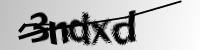
\includegraphics{ModeloRelatorio/figuras/3ndxd.png}
    \caption{Caption}
    \label{fig:captcha_exemplo}
\end{figure}

\begin{algorithm}{}
\caption{Reconhecimento de Captcha}
\label{alg:captcha}
    \begin{algorithmic}[1]
    \State simbolos $\leftarrow$ todos as letras do alfabeto em caixa baixa juntamente com os dígitos indo-arábicos
    \STATE num\_symbols $\leftarrow$ numero total de símbolos
    \State X,y $\leftarrow$ pré-processamento de dados (normalização dos dados, juntamente com outros ajustes pertinentes)
    \State X\_train, y\_train $\leftarrow$ X[:970], y[:, :970] (divide parte do dataset em treinamento)
    \State X\_test, y\_test $\leftarrow$ X[970:], y[:, 970:] (divide parte do dataset em teste)
    
    \State net $\leftarrow$ cria rede neural (por padrão, rede de cinco camadas, sendo um entrada, uma saída e o restante \textit{hidden}, ativada por ``relu'' e otimizada por ``rmsprop'')
    \State history $\leftarrow$ net.fit (ajuste de rede usando dataset de treino)
    \State net.evaluate(dataset de teste)

    \WHILE{sistema\_operacional.le\_imagens}
        \State realiza a predicao
    \ENDWHILE
    \end{algorithmic}
\end{algorithm}

O primeiro a ser discutido é o Keras. Keras é uma API de Deep Learning escrita em Python, rodando sobre a plataforma de Machine Learning TensorFlow. Foi desenvolvido com o objetivo de permitir experimentação rápida. Ser capaz de passar da ideia para o resultado o mais rápido possível é essencial para fazer uma boa pesquisa (fonte: https://keras.io/about/).

São importadas bibliotecas do python também como o "os", que serve para fazer chamadas no sistema operacional, o cv2 que é uma versão do OpenCV (Open Source Computer Vision Library) que, por sua vez, é uma biblioteca de software de visão computacional e Machine Learning de código aberto. O OpenCV foi desenvolvido para fornecer uma infraestrutura comum para aplicativos de visão computacional e acelerar o uso da percepção da máquina nos produtos comerciais (fonte: https://opencv.org/about/). 

A "string" que, como o nome indica, serve para manipulação de strings.
Por último, duas bibliotecas muito importantes para manipulação de dados e em algoritmos de Machine Learning: o numpy e o matplotlib. O NumPy é o pacote fundamental para a computação científica em Python. É uma biblioteca Python que fornece um objeto de matriz multidimensional, vários objetos derivados (como matrizes e matrizes mascaradas) e uma variedade de rotinas para operações rápidas em matrizes, incluindo matemática, lógica, manipulação de formas, classificação, seleção, I/O , transformadas discretas de Fourier, álgebra linear básica, operações estatísticas básicas, simulação aleatória entre outras operações (fonte: https://numpy.org/doc/stable/user/whatisnumpy.html).

Já o Matplotlib é uma biblioteca de visualização em Python para gráficos 2D de matrizes. é multiplataforma construída em matrizes NumPy e projetada para trabalhar com a pilha SciPy mais ampla. Ele nos permite acesso visual a grandes quantidades de dados em imagens, consistindo em vários gráficos, como linha, barra, dispersão, histograma etc .

\section{Resultados e Discussão}

% Testes: 

\textbf{Lista inicial}\\
análise de epochs
parada de fit
avaliar o dataset
se a precisão estiver baixa, alterar as camadas

XXXX

\section{Conclusões}

XXXX

%******************************************************************************
% Referências - Definidas no arquivo Relatorio.bib


\bibliographystyle{IEEEtran}

\bibliography{Relatorio}


%******************************************************************************

\vspace{20ex}

\vspace{3ex}

\end{document}
